\documentclass[main]{subfiles}
\begin{document}

%@@@@@@@@@@@@@@@@@@@@@@@@@@@@@@
% summarizes lecture 10
% author: Benjamin Ellenberger

\section{Ensemble Methods for Classifier Design}
Ensemble methods use multiple learning algorithms to obtain better predictive performance than could be obtained from any of the constituent learning algorithms. A machine learning ensemble refers only to a concrete finite set of alternative models, but typically allows for much more flexible structure to exist between those alternatives.\\
An ensemble is itself a supervised learning algorithm, because it can be trained and then used to make predictions. The trained ensemble, therefore, represents a single hypothesis. This hypothesis, however, is not necessarily contained within the hypothesis space of the models from which it is built. Thus, ensembles can be shown to have more flexibility in the functions they can represent. This flexibility can, in theory, enable them to over-fit the training data more than a single model would, but in practice, some ensemble techniques (especially bagging) tend to reduce problems related to over-fitting of the training data.\\

Empirically, ensembles tend to yield better results when there is a significant diversity among the models. Many ensemble methods, therefore, seek to promote diversity among the models they combine. Although perhaps non-intuitive, more random algorithms (like random decision trees) can be used to produce a stronger ensemble than very deliberate algorithms (like entropy-reducing decision trees). Using a variety of strong learning algorithms, however, has been shown to be more effective than using techniques that attempt to dumb-down the models in order to promote diversity. (Wikipedia)
\subsection{Advantages}
\paragraph{Computational:} They are easy to train.
\paragraph{Statistical:} Data randomization in the spirit of Bootstrap captures statistical dependencies between alternative hypotheses.
\(\rightarrow\) The classifier ensemble encodes uncertainty intervals in the hypothesis class (output space).
\todo[inline]{What does this mean?}
\subsection{Reminders}
\paragraph{Bias}Combining a set of estimators \(\pl{\hat f_1(x),\hat f_2(x),\ldots,\hat f_B(x)}\) by a simple average \(\hat f(x) = \frac{1}{B} \sum\limits_{i=1}^B \hat f_i(x)\) lets unbiased estimators remain unbiased.
\paragraph{Variance} Combining a set of \(B\) estimators by a simple average reduces the variance by a factor of \(\frac{1}{B}\) if bias remains unchanged.

\paragraph{Empirical error}
\[\pl{\hat{\mathcal{R}}_n (c) = \frac{1}{n} \#\{c(x_i) \neq y_i : 1 \leq i \leq n\}}\]
\paragraph{Expected error}
\[\pl{\mathcal{R}(c) = P\{c(x) \neq Y\}}\]
\paragraph{\((\epsilon,\delta)\) criterion}
\[\pl{P_{X,Y}\{\mathcal{R}(\hat c_n) \leq \mathcal{R}(c^{Bayes}) + \epsilon\} > 1 - \delta}\]
\subsection{Empirical Risk Minimization Principle}
Select classifier \(c \in \mathcal{C}\) with the smallest error on the training data \(\pl{\mc{Z} = \{(x_1,y_1),\ldots,(x_n,y_n)\}}\):
\[\pl{c^\ast_n \argmin_{c\in \mc{C}} \hat{\mc{R}}_n (c) = \argmin_{c \in \mc{C}} \frac{1}{n} \#\{c(x_i) \neq y_i:~1 \leq i \leq n\}}\]

Goal: Derive a distribution independent bound for 
\[\pl{P\{\mathcal{R}(\hat c^\ast_n)-\inf\limits_{c\in\mathcal{C}}\underbrace{\mathcal{R}}_{\hidewidth=P(c(X)) \neq Y\hidewidth}(c) > \epsilon\} < \delta}\]
\subsection{Probably Approximately Correct (PAC) Learning}
\subsubsection{Strong and Weak Learning}
Assumption: Restricted classifier \(\pl{c \in \mathcal{C}}\) (hypothesis class).
Classification Error for empirically determined classifier \(\pl{\hat{c}}\)
\[\pl{P \left\{\mathcal{R}(\hat{c})-\inf\limits_{c \in \mathcal{C}} \mathcal{R}(c) > \epsilon\right\} < \delta (\ast)}\]
\paragraph{Strong PAC Learning} requires to achieve an arbitrarily small error \(\epsilon\) with high probability \(1 - \delta\).

\paragraph{Weak PAC Learning} demands that \((\ast)\) holds for ‘large’, but ‘better than chance’ \(\epsilon\). Weak learning has to achieve a non trivial error rate, i.e., the rate has to be bounded away from the chance \(\epsilon\)-value. 

\subsection{Motivation for Ensemble Methods}
Train several sufficiently diverse predictors, i.e., classifiers or regressors and use an aggregation scheme to produce a valid solution with low bias and variance.

\subsubsection{Weak Learners used for bagging or boosting}
\begin{itemize}
\item \textbf{Stumps}: Single axis parallel partition of space
\item \textbf{Decision trees}: Hierarchical partition of space
\item \textbf{Multi-layer perceptrons}: General non-linear function approximators
\item \textbf{Radial basis functions}: Non-linear expansions based on kernels
\end{itemize}

\subsubsection{Combining classifiers}

Input: A pool of binary classifiers \(\pl{c_1 (x), c_2 (x), \ldots, c_B (x)}\)
Objective: Infer a composite classifier with weights \(\pl{{\alpha_b }^B_{b=1}}\)
\[\pl{
\hat{c}_B (x) = \sgn\left(\sum\limits^B_{b=1} \alpha_b c_b (x)\right)
}\]
\paragraph{Question:} When can this procedure succeed? It works by adding enough diversity among the classifiers

\paragraph{Diversity:} 
\begin{itemize}
\item Use different subsets of the data for each \(c_b\)
\item Use different features
\item Decorrelate classifiers during training
\end{itemize}

\subsection{Bagging}
Bagging or bootstrap aggregation combines several classifiers which have been trained on random subsamples (with replacements) of the data.
(Breiman, 1996)

\paragraph{Idea:}
Generate diversity in classifier pool by training on different, e.g. bootstrapped subsets!

\textbf{Bootstrap sample:} Given \(Z = {(x_1 , y_1 ), \ldots, (x_n , y_n )}\) generate \(Z\) by choosing i.i.d. pairs with replacement.\\\\

INPUT: data \(\pl{(x_1 , y_1 ), \ldots , (x_n , y_n )}\)
OUTPUT: classifier with majority vote of \(\pl{\{c_1 , c_2 , \ldots , c_B \}}\)
\begin{enumerate}
\item \textbf{for} b = 1 to B \textbf{do}
\item \hspace{0.5em}\(pl{\mc{Z}^{\ast b}}\) = b-th bootstrap sample from \(\pl{\mc{Z}}\)
\item \hspace{0.5em}Construct classifier \(c_b\) based on \(\pl{\mathcal{Z}^{\ast b}}\)
\item \textbf{end for}
\item \textbf{return} ensemble classifier \(\pl{\hat{c}_B (x) = \sgn\left(\sum\limits^B_{b=1} c_b (x)\right)}\)
\end{enumerate}

\subsubsection{Why does Bagging work?}
\paragraph{Covariances small:} Due to using different subsets for training
\paragraph{Variances similar:} Estimator from each sub-sample behaves similarly (on average)
\paragraph{Biases:} Weakly affected

More elaborate explanation - B\"uhlmann and Yu 1999

\textbf{Takeaway Message:}
It is advantageous to reduce dependence between component estimators
\subsection{Decision Trees}
Decision tree learning is the construction of a decision tree from class-labeled training tuples. A decision tree is a flow-chart-like structure, where each internal (non-leaf) node denotes a test on an attribute, each branch represents the outcome of a test, and each leaf (or terminal) node holds a class label. The topmost node in a tree is the root node.

There are many specific decision-tree algorithms. Notable ones include:

\begin{itemize}
\item \textbf{ID3} (Iterative Dichotomiser 3)
\item \textbf{C4.5} (successor of ID3)
\item \textbf{CART} (Classification And Regression Tree)
\item \textbf{CHAID} (CHi-squared Automatic Interaction Detector). Performs multi-level splits when computing classification trees.
\textbf{MARS:} extends decision trees to handle numerical data better.
\end{itemize}

The term Classification And Regression Tree (CART) analysis is an umbrella term used to refer to both of the following procedures:

\begin{itemize}
\item \textbf{Classification tree analysis} is when the predicted outcome is the class to which the data belongs.
\item \textbf{Regression tree analysis} is when the predicted outcome can be considered a real number (e.g. the price of a house, or a patient’s length of stay in a hospital).
\end{itemize}

Trees used for regression and trees used for classification have some similarities - but also some differences, such as the procedure used to determine where to split.\\\\

\begin{figure}[H]
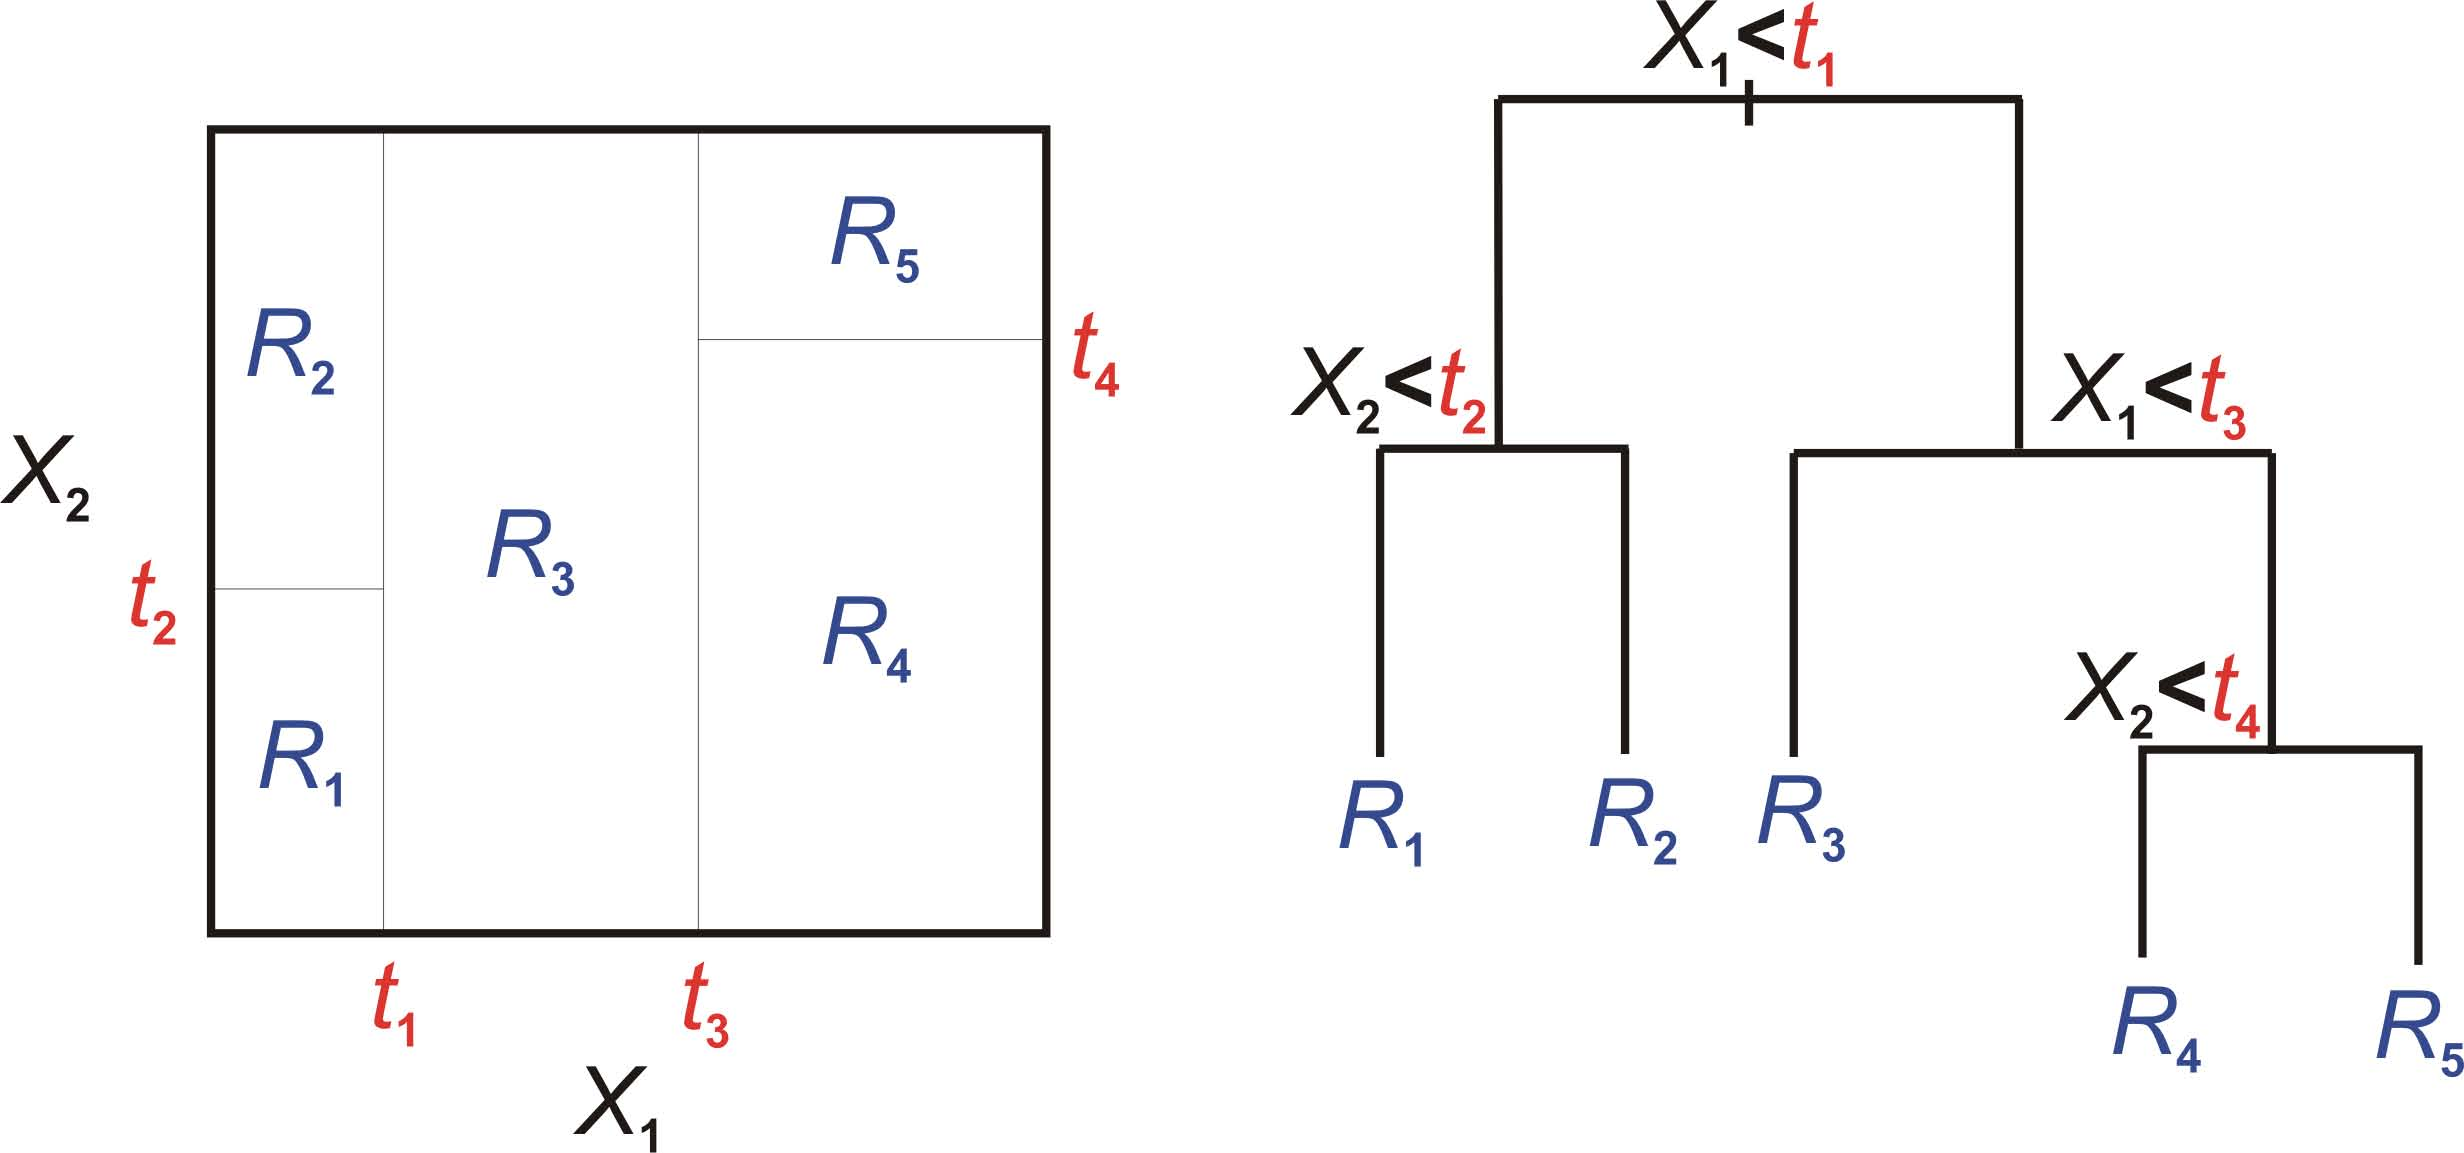
\includegraphics[width=0.8\linewidth]{figs/decision-tree.png}
\caption{The data space is recursively partitioned into dichotomies. Example for \(( X_1 , X_2 ) \in \R^2\) with partitions \(R_i\) and thresholds \(t_j\)}
\end{figure}

\begin{figure}[H]
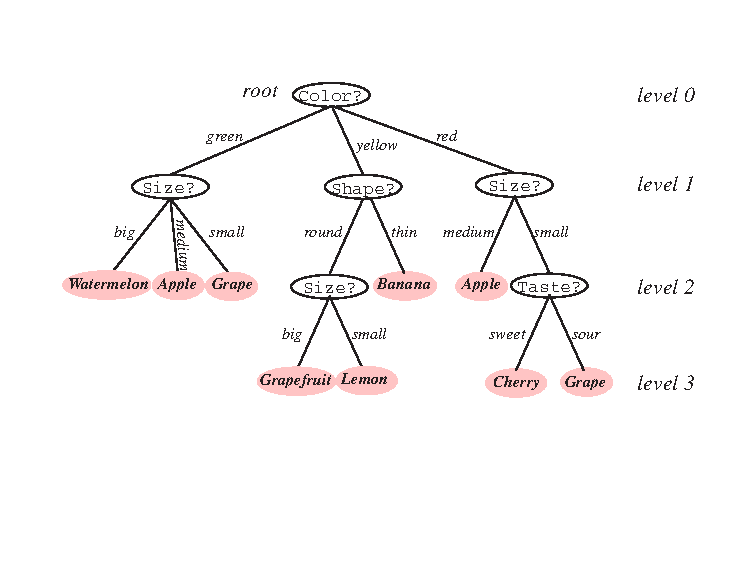
\includegraphics[width=0.8\linewidth]{figs/classification-decision-tree.pdf}
\caption{Classification of fruits}
\end{figure}

\subsection{Random Forests}
Random forests are an ensemble learning method for classification, regression and other tasks, that operate by constructing a multitude of decision trees at training time and outputting the class that is the mode of the classes (classification) or mean prediction (regression) of the individual trees. Random forests correct for decision trees' habit of overfitting to their training set.

The algorithm for inducing a random forest combines the "bagging" idea and the random selection of features in order to construct a collection of decision trees with controlled variance.

\paragraph{Strategy for bagging trees} Grow a sufficiently deep decision tree to reduce bias \(\rightarrow\) noisy classifier \(\rightarrow\) average to enhance robustness.

\paragraph{Classification of a new sample} Let \(\hat{c}_b (x)\) be the class prediction of the \(b^{th}\) random forest tree. Then, the random forest classification yields
\[\pl{\hat{c}^B_{rf} (x) = \text{majority vote}\{\hat{c}_b (x)\}^B_{b=1}}\]

\begin{enumerate}
\item \textbf{for} b = 1 to B \textbf{do}
\item \hspace{0.5em} draw a bootstrap sample \(\pl{\mathcal{Z}^\ast = \{(X^\ast_1 , Y^\ast_1 , \ldots , (X^\ast_n , Y^\ast_n )\}}\) of
size n from the training data \(\mathcal{Z}\);
\item \hspace{0.5em}//generatation  of a random forest tree
\item \hspace{0.5em} grow a random forest tree \(\hat{c}_b (x)\) to the bootstrapped data, by recursively repeating
\item \hspace{0.5em}// the following steps for each leaf until the minimum node size \(n_min\) is reached.
\item \hspace{0.5em}\textbf{repeat}
\item \hspace{1em}select m variables at random from p variables
\item \hspace{1em}\((m \approx \sqrt{p})\)
\item \hspace{1em}pick the best variable/split-point among the m selected
variables
\item \hspace{1em}split the node into two daughter nodes
\item \hspace{0.5em}\textbf{until} node size \(n_min\) is reached
\item \textbf{end for}
\item return Output the ensemble of trees \(\{\hat{c_b} (x)\}^B_{b=1}\)
\end{enumerate}

\subsection{Boosting}
Boosting is an approach to machine learning based on the idea of creating a highly accurate, excellent, complex classifier by making an adaptive combination of many relatively weak and inaccurate rules with sufficient diversity. (R. Shapire, Explaining AdaBoost. Springer, 2013.) It is built from the base class of simple classifiers such as perceptrons, decision stumps, axis parallel splits etc.

Output classifier: \[\pl{
\hat{c}_B (x) = \sgn\left(\sum\limits^B_{b=1} \alpha_b c_b (x)\right)
}\]

\begin{figure}[H]
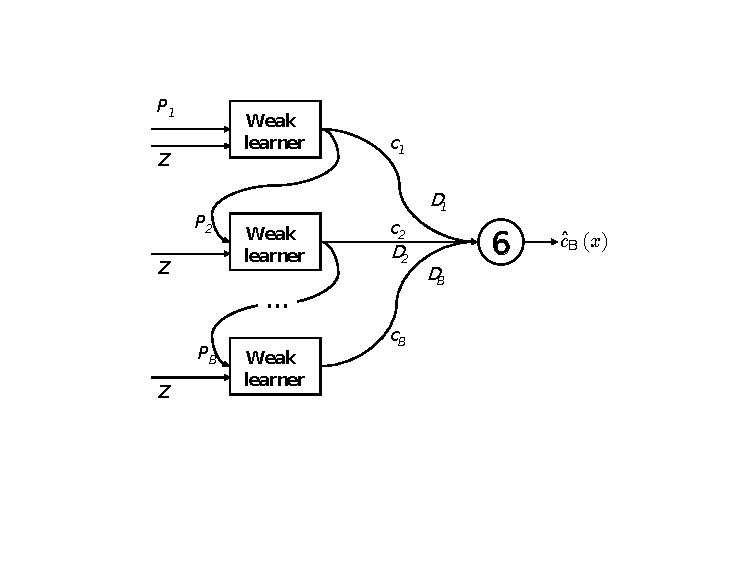
\includegraphics[width=0.8\linewidth]{figs/adaboost.pdf}
\caption{Boosting in form of AdaBoost is an ensemble method with error sensitive reweighting of the classifiers (Freund \& Shapire, 1995).}
\end{figure}

Weak Learner: \[\pl{\epsilon_b \triangleq \frac{\sum\limits^n_{i=1} w^{(b)}_i \I_{\{\underbrace{c_b(x_i)}_{\hidewidth\text{binary}\hidewidth}\neq y_i\}}}{\sum\limits^n_{i=1}w^{(b)}_i}}\]


\subsection{Arcing}
Arcing or adaptive reweighting and combining is an extension of bagging introduced by Breiman (1998)
\subsection{Exponential Loss}
\end{document}